\section{Durchführung}
\label{sec:Durchführung}

\subsection{Aufbau}
\label{sec:Aufbau}

\begin{figure}[H]
\centering
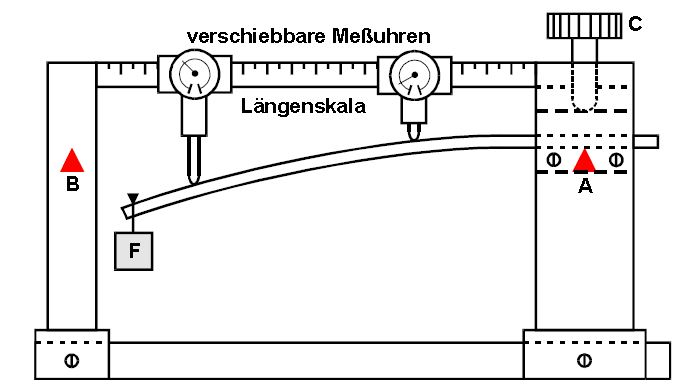
\includegraphics[width=\linewidth-30pt,height=\textheight-30pt,keepaspectratio]{Text/Bilder/Aufbau.png}
\caption{Schematischer Aufbau des Prismenspektralapparates \cite[24]{sample}.}
\label{fig:aufbau}
\end{figure}

Der in Abbildung \ref{fig:aufbau} dargestellte Aufbau besteht aus einem fest angebrachten Kollimatorrohr, einem drehbaren Prisma und einem bewegbaren Fernrohr.
Licht einer Quecksilber-Cadmium Lampe wird durch das Kollimatorrohr auf das Prisma geworfen, sodasss die Spektrallinien mithilfe des Fernrohrs analysiert werden können.
Der Aufbau wird für die folgenden Versuchsteile verwendet.

\subsection{Bestimmung des Winkels zwischen den brechenden Oberflächen des Prismas}

Zur Bestimmung des bereits in Kapitel \ref{sec:MessPhi} erwähnten Winkels $\phi$  wird das Prisma mit einer seiner brechenden Kanten auf das Kollimatorrohr ausgerichtet.
Die Winkel  $\phi_l$ und $\phi_r$ werden mithilfe des Fernrohr bestimmt, indem die Ablenkung der reflektierten Stahlen ausgemessen wird.
Der Messvorgang wird für leicht veränderte Ausrichtungen des Prismas wiederholt.

\subsection{Bestimmung der Brechungswinkel für die Spektrallinien einer Quecksilber-Cadmium Lampe}

In diesem Versuchsteil wird der Brechungswinkel $\eta_i$ bestimmt. Dazu wird das Prisma entsprechend Abbildung \ref{fig:eta1} ausgerichtet, sodass
eine der brechenden Kanten auf das Kollimatorrohr zeigt.
Der Winkel $\Omega_{l_i}$ wird daraufhin mithilfe des Fernrohrs für die einzelnen Spektrallinien der Quecksilber-Lampe bestimmt.
Dabei wird dieses so gedreht, dass das Spaltbild des gebrochenen Strahlenbündels mit dem des reflektierten Strahlenbündels zusammenfällt.
Ebenso ist auf die Ausrichtung des Fadenkreuzes zu achten. Dieses soll möglichst genau auf der Spektrallinie liegen.
Die Messung wird mit einer Spiegelsymmetrischen Stellung des Prismas wiederholt, um  $\Omega_{r_i}$ zu bestimmen.
